\documentclass[11pt]{report}

\usepackage{graphicx}
\usepackage{listings}
\usepackage{color}
\usepackage{placeins}

\setlength{\topmargin}{0in}
\setlength{\headheight}{0in}
\setlength{\headsep}{0in}
\setlength{\textheight}{9.0in}
\setlength{\textwidth}{6.5in}
\setlength{\evensidemargin}{0in}
\setlength{\oddsidemargin}{0in}


\begin{document}

\title{Implementing Multiple Blocks within MPAS Framework}
\author{}

\maketitle
\tableofcontents


%%%%%%%%%%%%%%%%%%%%%%%%%%%%%%%%%%%%%%%%
%
% Introduction
%
%%%%%%%%%%%%%%%%%%%%%%%%%%%%%%%%%%%%%%%%
\chapter{Introduction}

Previously several projects have been worked on with the end goal of supporting
multiple blocks. These tasks are described below.

\begin{enumerate}

\item Update/extend the fundamental derived types in mpas\_grid\_types.F.                                
   In order for other parts of the infrastructure to handle multiple                                
   blocks per task in a clean way, we'll need to be able to pass a head                             
   pointer to a field into a routine, and have that routine loop through                            
   all blocks for that field, with information about which cells/edges/vertices                     
   in that field need to be communicated.                                                           
                                                                                                    
\item Decide on a new MPAS I/O abstraction layer, which will provide a                                
   high-level interface to the PIO layer for the rest of MPAS. This layer                           
   should work with blocks of fields, and make it possible to define an                             
   arbitrary set of I/O streams at run-time.                                                        
                                                                                                    
\item Add a new module to parse a run-time I/O configuration file that                                
   will describe which fields are read or written to each of the I/O                                
   streams that a user requests via the file. This module will make calls                           
   to the new MPAS I/O layer to register the requested fields for I/O in                            
   the requested streams.                                          
   
\item Update the mpas\_dmpar module to support communication operations on                              
   multiple blocks per task. This will likely involve revising the                                  
   internal data structures used to define communication of cells                                   
   between tasks, and also require revisions to the public interface                                
   routines themselves.                                                                             
                                                                                                    
\item Modify the block\_decomp module to enable a task to get a list of                                 
   cells in more than one block that it is to be the owner of.                                      
   Implemented in the simplest way, there could simply be a namelist                                
   option to specify how many blocks each task should own, and the                                  
   block\_decomp module could look for a graph.info.part.n file, with                                
   n=num\_blocks\_per\_task*num\_tasks, and assign blocks k, 2k, 3k, ...,                               
   num\_blocks\_per\_task*k to task k.    

\end{enumerate}                                                             

This document related to tying all of these projects together, and allowing
MPAS to run with multiple blocks per MPI process.

As an example of what running with multiple blocks means, currently MPAS is
allowed to run with 1 block per process. This means prior to running MPAS a
decomposition of cells needs to be determined. This decomposition tells each
MPI process which cells it owns. So, under the current framework the number of
decompositions have to be equal to the number of MPI tasks used to run the job. 

After this project is completed, a user should be able to specify the use of a
decomposition that does not have an equal number of blocks as the number of
processors the job is run with. Typically this would be used to allow more than
one block per processor, but could theoretically be used to run having some
processors not have any blocks.

The goal with this project is to allow exploration of OpenMP directives, and
test performance using different block sizes. Allowing multiple blocks per
processor could increase cache reuse and allow a performance increase.

This work is currently being performed under
branches/omp\_blocks/multiple\_blocks and all source code changes can be
examined there.

%%%%%%%%%%%%%%%%%%%%%%%%%%%%%%%%%%%%%%%%
%
% Requirements
%
%%%%%%%%%%%%%%%%%%%%%%%%%%%%%%%%%%%%%%%%
\chapter{Requirements}

There are significant changes to MPAS' framework that have to be made in order
to support multiple blocks. A list of requirements that determine these changes
are listed below, with the reasons for these requirements written below them.

\begin{itemize}
	\item Block creation must be robust, and handle an arbitrary number
		of blocks per processor.

	\item Blocks should be created using the derived data types created in an
		earlier project, promoting the use of field data types rather than
		simple arrays.

	\item Block creation routines should be created with an arbitrary number of
		halos assumed, although the default is currently two.

	\item All block communication routines should be able to handle shared
		memory copies.

	\item Exchange list creation should be performed at the block/field level.

	\item Block creation code should be isolated from the rest of MPAS code.
\end{itemize}

Blocks per processor should be allowed to be any non-negative number, including
zero. This could be useful if a user wanted the ability to specify certain
processors to do certain tasks, without doing any actual computation work on
blocks. Although the user would have to give an explicit block to proc
decomposition in order to have this ability used.

In the creation of blocks, field data types should be used in place of simple
arrays to promote the use of internal derived data types that are used
elsewhere within MPAS. This will allow similar techniques to be identified by
developers of cores, and allow a similar work flow with variables and fields
within all of MPAS.

Although fields currently are restricted to having two halo layers, at some
point in the future we might like to be able to extend halo layers or even have
different halo layers on each field. In order to make this task easier to
accomplish in the future block creation routines need to be able to create an
arbitrary number of halo layers. 

When two blocks are neighboring on a single processor shared memory copies
could be used for halo exchanges and other sorts of block-to-block
communications rather than using MPI send/recv routines.

Exchange lists are limited in their functionality by the fact that the only
information they have refer to the other processor/block involved in the
communication. For example, if processor 0 owns block 0 and this has to send
information from 15 cells to processor 2 block 5 then the send list for block 0
only gives the information on where it has to send the information, while the
receive list on block 5 gives information on where to receive the information
from. Because of this, exchange lists have to be created on a per block basis,
and linked to a specific block. This way each block knows which cells it's
supposed to send/recv/copy to/from another block. Each field and block have
their own exchange lists, so the creation of exchange lists should place them
within these already existing structures.

%%%%%%%%%%%%%%%%%%%%%%%%%%%%%%%%%%%%%%%%
%
% Design
%
%%%%%%%%%%%%%%%%%%%%%%%%%%%%%%%%%%%%%%%%
\chapter{Design}

Only a small amount of design has been completed thus far. So, all information
in this section should be regarded as a work in progress for now. As a visual
for the design process, the proposed module layout can be seen in figure
\ref{fig:module_layout}.

\begin{figure}[H!]
	\centering
	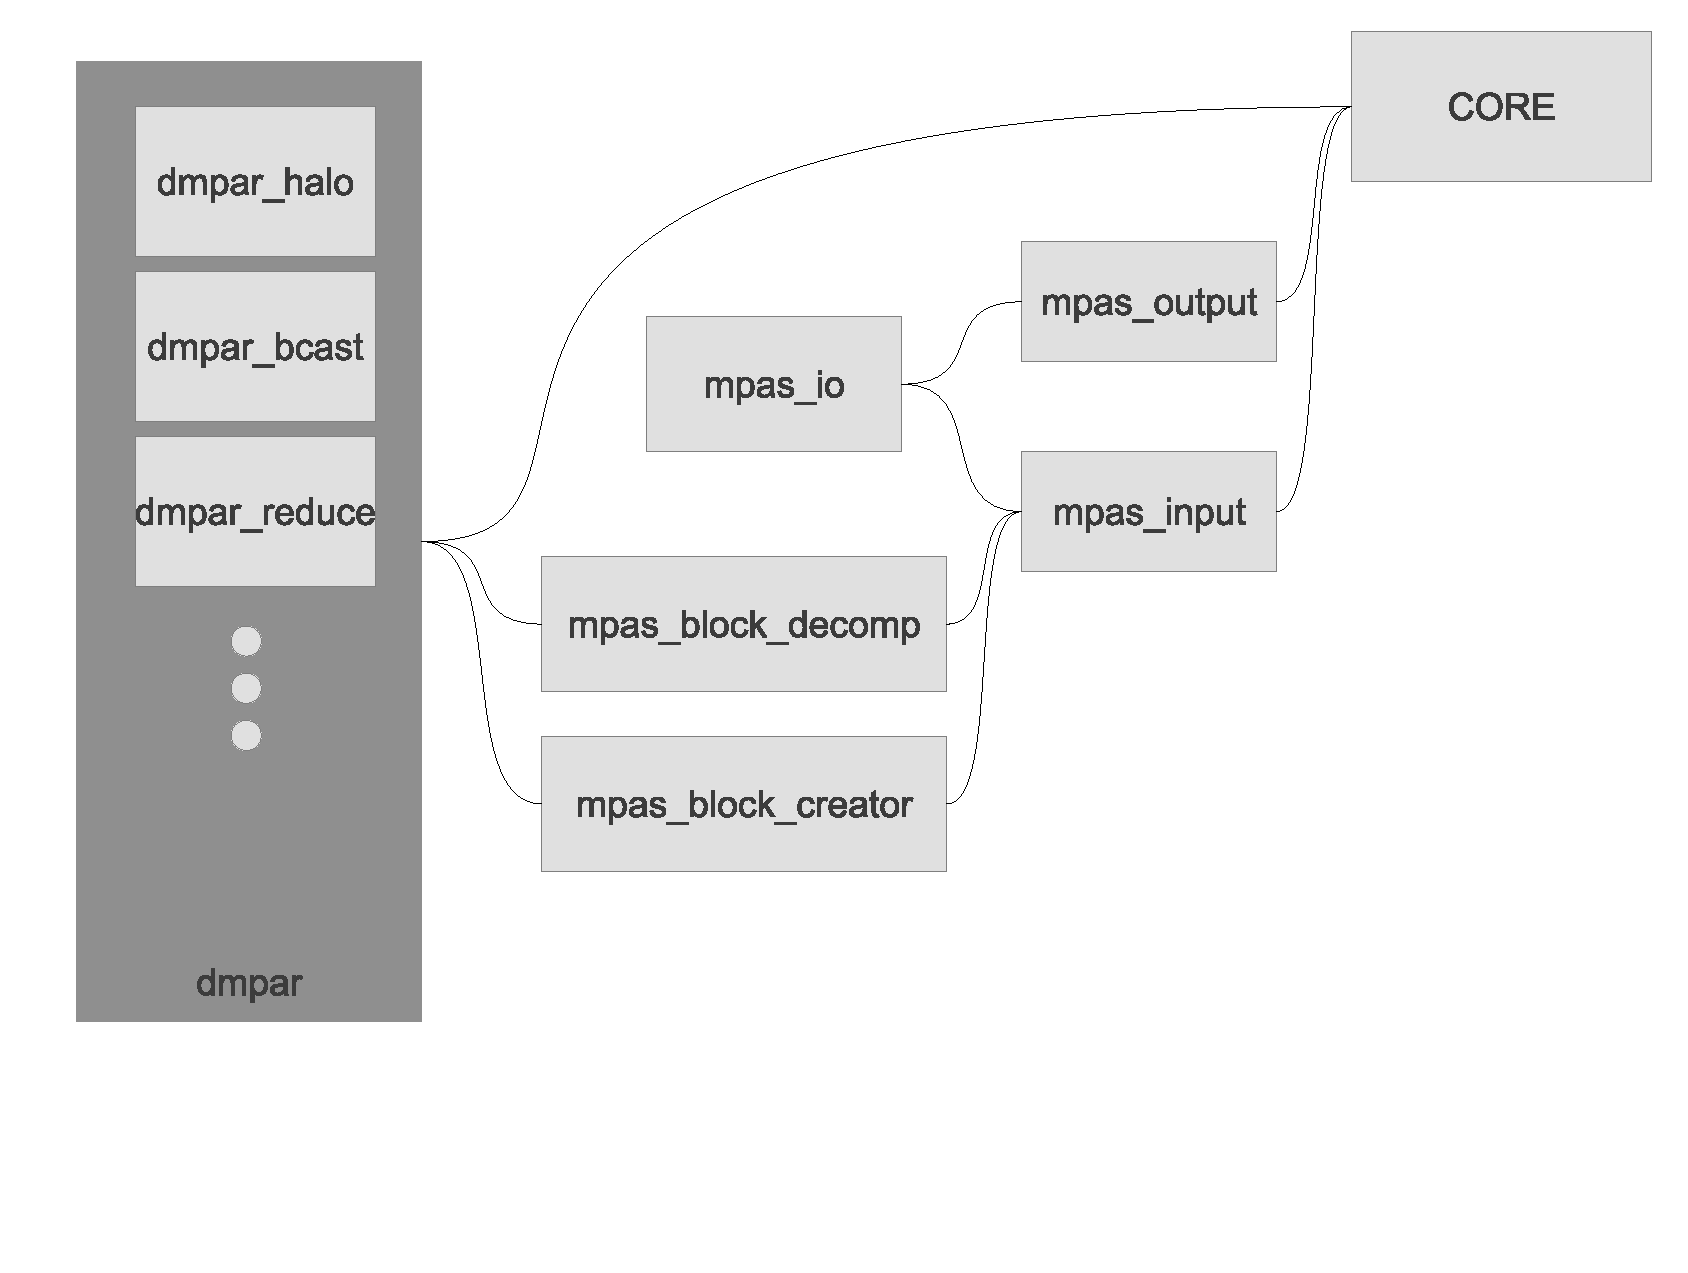
\includegraphics[scale=0.4]{DesignLayout.eps}
	\caption{Layout of modules for input/output with multiple blocks}
	\label{fig:module_layout}
\end{figure}

The changes made to mpas framework can be seen in the following sections.

\section{Changes in mpas\_dmpar}
This section covers the changes, and the new functionality of the changes that
were made within the mpas\_dmpar.F file. The first major change, is that dmpar
is renamed to comm meaning communications. 

\subsection{Data types}
Previously the derived data type mpas\_exchange\_list was used to create a linked list which represented an exchange list (send or receive). Exchange lists have been modified from their original state to have the following structure.
\begin{lstlisting}[language=fortran,escapechar=@,frame=single]
type mpas_exchange_list
 integer :: endPointID
 integer :: nlist
 integer, dimension(:), pointer :: srcList
 integer, dimension(:), pointer :: destList
 type (mpas_exchange_list), pointer :: next
end type mpas_exchange_list
\end{lstlisting}

Within this structure endPointID can be either a blockID (for local copy) or a procID for mpi send/recv, nList represents the number of elements to be communication within this exchange list, srcList and destList represent the information for packing and unpacking data into buffers or for local copies from/to arrays.

Seeing as the exchange lists no longer contain an array for the communication buffers a new data type was created which can be seen below.

\begin{lstlisting}[language=fortran,escapechar=@,frame=single]
type mpas_communication_list
 integer :: procID
 integer :: nlist
 real (kind=RKIND), dimension(:), pointer :: rbuffer
 integer, dimension(:), pointer :: ibuffer
 integer :: reqID
 type (mpas_communication_list), pointer :: next
end type mpas_communication_list
\end{lstlisting}

An mpas\_communcation\_list is only intended to be used for mpi communications. These have to be created and destroyed each time a communcation is performed. Within the structure, procID represents the other endPoint's processor ID in the communication, nList is the number of elements to be communicated within the buffer, rbuffer and ibuffer are the pointers for the buffer of either integers or reals, reqID represents the mpi communcation id, and next creates a linked list.

Two other data structures are created to allow multi halo exchange lists, and to allow pointers to be swapped easily using them.

\begin{lstlisting}[language=fortran,escapechar=@,frame=single]
type mpas_exchange_list_pointer
 type (mpas_exchange_list), pointer :: exchList
end type mpas_exchange_list_pointer

type mpas_multihalo_exchange_list
 type (mpas_exchange_list_pointer), dimension(:), pointer :: halos
end type mpas_multihalo_exchange_list
\end{lstlisting}

Combining these four structures allows local and mpi communications to occur smoothly.

\subsection{mpas\_comm\_get\_exch\_list}
The old routine named mpas\_dmpar\_get\_owner\_list is now renamed to mpas\_comm\_get\_exch\_list. This routine is meant to create send, receive, and copy lists to send data from one processor to another. During initialization it's used for the allToAll communication routines (which will be described below) but within cores it's almost exclusively used for halo exchanges.

It works by creating two lists of element id's (typically cells, edges, or vertices). One of these lists is owned elements while the other is needed elements. The needed list is communication round robin style to each processor until it comes back to the original processor. Each processor marks a needed element in the list as owned if it owns it. This way the processor that needs the element knows who it's supposed to receive the element from.

During the round robin communications send lists are created as needed elements are marked as owned. After the round robin communications are finished receive lists are created. And after receive lists are created copy lists are created in a similar fashion to send lists.

\subsection{allToAll routines}
mpas\_comm provides a set of allToAll routines intended to distribute a field from one processor to one or more other processors. In this case, the sending information is supposed to include the 0 halo elements. In contrast to the exch\_halo routines which are intended to only communication 1+ halo elements.

A pseudocode version of the allToAll routines can be seen below.
\begin{lstlisting}[language=fortran,escapechar=@,frame=single]
loop over fieldOut list
  loop over recvList for specific field
    create new communication list if needed
  end loop
end loop

allocate recvList buffers and initiate mpi_irecvs

loop over fieldIn list
  loop over sendList for specific field
    create new communication list if needed
  end loop
end loop

allocate sendList buffers, copy data into buffer
  initiate mpi_isends

loop over fieldIn list
  loop over copyList for specific field
    loop over fieldOut list
      if fieldOut % blockID == copyList % endPointID
        use copy list to copy from fieldIn to fieldOut
	  end if
	end loop
  end loop
end loop

wait for mpi_irecvs
  unpack buffer into fields

wait for mpi_isends

destroy buffers
\end{lstlisting}

\subsection{exch\_halo routines}
mpas\_comm provides a set of halo exchange routines intended to distribute a set of 0 halo elements to other blocks that have them in their 1+ halo regions.

A pseudocode version of the halo exchange routines can be seen below.
\begin{lstlisting}[language=fortran,escapechar=@,frame=single]
loop over field list
  loop over recvList for specific field
    create new communication list if needed
  end loop
end loop

allocate recvList buffers and initiate mpi_irecvs

loop over field list
  loop over sendList for specific field
    create new communication list if needed
  end loop
end loop

allocate sendList buffers, copy data into buffer
  initiate mpi_isends

loop over field list
  loop over copyList for specific field
    loop over field list
      if field % blockID == copyList % endPointID
        use copy list to copy from fieldIn to fieldOut
	  end if
	end loop
  end loop
end loop

wait for mpi_irecvs
  unpack buffer into fields

wait for mpi_isends

destroy buffers
\end{lstlisting}

\subsection{copy routines}
mpas\_comm provides a set of routines intended to copy a field from the header block in a list of owned blocks to all other blocks in the list. These are needed during initialization to copy non-decomposed fields (fields that don't include the nCells, nEdges, or nVertices as a dimension) to all owned blocks.

\subsection{Utility routines}
In addition to communcation routines, mpas\_comm provides utility routines for the initialization and destruction of all derived data types discussed above.

\section{mpas\_block\_creator.F}
mpas\_block\_creator provides a new module for mpas that is used to create computational blocks. Given the information of a 0 halo, these routines create the 1+ halo regions for cells, edges, and vertices. They also initialize the list of local blocks.

\subsection{Cell Routines}
Routines to setup cell fields within a block are:
\begin{lstlisting}[language=fortran,escapechar=@,frame=single]
mpas_block_creator_setup_blocks_and_0halo_cells
mpas_block_creator_build_0halo_cell_fields
mpas_block_creator_build_cell_halos
\end{lstlisting}

These routines should be called in this order to properly setup the 0-1+ halo of cells. However, the build\_cell\_halos routine should not be called until all 0 halo fields are setup (including edges and vertices).

\subsection{Edge/Vertex Routines}
Routines used to setup edge/vertex fields within a block are:
\begin{lstlisting}[language=fortran,escapechar=@,frame=single]
mpas_block_creator_build_0_and_1halo_edge_fields
mpas_block_creator_build_edge_halos
\end{lstlisting}

As mentioned in the cell routine section, the 0-1 halos of edges and vertices should be setup prior to setting up the 1+ halos of cells.

\subsection{Utility Routines}
Finally, two routines are provided to finalize the block initialization, and to re-index all fields in a block.

\begin{lstlisting}[language=fortran,escapechar=@,frame=single]
mpas_block_creator_finalize_block_init
mpas_block_creator_reindex_block_fields
\end{lstlisting}

These routines complete the block creation processor, and provide the rest of a model with a list of fully setup blocks to compute on.

\section{mpas\_io\_input changes}
Within mpas\_io\_input the main mpas\_input\_state\_for\_domain routine has been trimmed significantly to make use of the new mpas\_block\_creator module the portions of the routine that were not able to be moved into the block\_creator module were moved to new routines within the io\_input module.

This module also makes use of the new communication routines from mpas\_comm, as well as some routines in mpas\_block\_decomp.

The new routines provided to clean up mpas\_input\_state\_for\_domain are:
\begin{lstlisting}[language=fortran,escapechar=@,frame=single]
mpas_io_setup_cell_block_fields
mpas_io_setup_edge_block_fields
mpas_io_setup_vertex_block_fields
\end{lstlisting}
These routines are intended to read in contiguous chunks of data that can then be communication between processors.

\section{mpas\_grid\_types changes}
Within mpas\_grid\_types, utility routines are created to deallocate fields. This is used within mpas\_io\_input for fields that need to be linked similarly to block, but are not part of the block data structure.

In addition to utility routine additions, a pointer provis was created within the block\_type. provis is intended to be a scratch state. This can be used within time integration routines that require an additional time level, without having to modify the number of time levels within state. 

\section{Namelist changes}
With the addition of multiple blocks in the framework of mpas, the decomposition namelist section will be made use of. This section provides the following namelist options.
\begin{lstlisting}[language=fortran,escapechar=@,frame=single]
config_block_decomp_file_prefix
config_number_of_blocks
config_explicit_proc_decomp
config_proc_decomp_file_prefix
\end{lstlisting}

The prefix options are used to specify the prefixes on decomposition graph files used to create blocks, and determine which blocks are owned by which processors, config\_number\_of\_blocks determines how many blocks the simulation is supposed to be run with, and config\_explicit\_proc\_decomp is a logical flag which determines if mpas should look for a graph file describing how blocks should be distributed between processor, or if it should round robin assign blocks to processors.

In addition to the decomposition section changes, the model sections (like sw\_model) now has a new namelist option:

\begin{lstlisting}[language=fortran,escapechar=@,frame=single]
config_num_halos
\end{lstlisting}

This namelist flag determines how many halo layers each block should have on cells. The halo layers for edges and vertices are nHaloLayerCells+1, or config\_num\_halos + 1.

\chapter{Testing}
**NOTE**
All of the testing described in this section relates only to the ocean core.
Other core developers may test this with similar procedures but different
simulations. \\

The end goal from this project is to provide a framework that allows
bit-for-bit reproduction of data using an arbitrary combination of blocks and
processor numbers.

Using this goal to define a testing strategy implies a good test would be
exploring bit-for-bit reproduction of output data using the three following
simulations:
\begin{itemize}
	\item Current trunk simulation run with 8 processors and 8 blocks (1 block per proc).
	\item Finished branch simulation run with 8 processors and 8 blocks (1 block per proc).
	\item Finished branch simulation run with 1 processor and 8 blocks (8 blocks per proc).
	\item Finished branch simulation run with 2 processors and 8 blocks (4 blocks per proc).
\end{itemize}

If all of these simulations produce bit-for-bit output then testing can move on
to a set of larger scale simulations.

\begin{itemize}
	\item Current trunk 15km simulation with 1200 processors and 1200 blocks (1 block per proc).
	\item Finished branch simulation with 1200 processors and 1200 blocks (1 block per proc).
	\item Finished branch simulation with 600 processors and 1200 blocks (2 blocks per proc).
	\item Finished branch simulation with 24 processors and 1200 blocks (50 blocks per proc).
\end{itemize}

After these final four simulations show bit-for-bit output then the project can
be deemed as completed.

\chapter{Appendix - Use of exchange/communication lists}
This chapter will describe the use of exchange and communication lists.

To begin, exchange lists have two uses. First copyLists will be described,
followed by send/recvLists.

copyLists are attached to the block sending the data, and there is no matching
list on the receiving end. Within the copyList, the endPointID variable
represents a blockID giving the local id to the block on the other end of the
communication, nList is the total number of elements that need to be copied,
srcList is the list of indices to take this data from out of the owning field's
array, and destList is the list of indices to put this data into the needing
field's array. 

In using copyLists, first a search over blocks needs to be preformed
to find the matching block for the communication. After that the elements
listed in srcList are copied into the elements listed in destList. After which,
the shared memory copy is complete.

The second use case relates to send/recvLists. sendLists are attached to
sending blocks, while recvLists are attached to receiving blocks. Within both
of these, endPointID refers to a processor id, and nList refers to the number
of elements a specific block should expect to communicate. In a sendList,
srcList describes the indices to pull data out from the owning field's array
while destList descibes the indices to put that data into a communication
list's buffer. In a recvList, srcList describes the indices to pull the data
out of the buffer, while destList describes the indices to put that data into
the needing field's array.

In order to use these, each side of the communication does something different.
Before describing the use of send and recv lists, communication lists need to
be explained.

A communication list describes aggregated communications between processors.
These provide an easy to use framework to allow communications to occur
processor by processor as opposed to block by block. Since communication lists
only relate to MPI communications, the only ID within the type is procID. nList
refers to the number of elements in the buffer, while rbuffer and ibuffer
provide deallocated arrays to put reals or integers in the buffer, and reqID
provides a variable to store MPI communication ID's to use when calling
MPI\_Wait.

In order to perform a send an receive, first a processor needs to build the
buffers, or communication lists. To begin the fields relating to the specific
communication are looped over, and the total number of elements to each
processor are stored in order to build a communication list for that processor.
After this step, the communication list buffers are allocated relating to their
nList varibles. Buffers need to be created both on the sending and receiving
side. After the buffers are created, the sending field copies all of it's data
into the array. The buffer is then sent, and on the receiving end the receiving
field unpacks all of the data into it's arrays.
\end{document}
